\documentclass[12pt,a4paper]{report}
\usepackage[T1]{fontenc}
\usepackage{lmodern}
\usepackage{anyfontsize}
\usepackage[a4paper, top=1in, bottom=1in, left=1in, right=1in]{geometry}
\usepackage{graphicx}
\usepackage{setspace}
\usepackage{titlesec}
\usepackage{ragged2e}
\usepackage{enumitem}
\usepackage{tikz}
\usepackage{longtable}
\usepackage{array}
\usepackage{booktabs}
\usepackage{hyperref}
\usepackage{xcolor}
\usepackage{float}
\usepackage{caption}
\usepackage{subcaption}
\usepackage{fancyhdr}
\usepackage{pgfplots}
\pgfplotsset{compat=1.18}

\usetikzlibrary{shapes.geometric, arrows.meta, positioning, calc, fit, backgrounds}

% Color definitions
\definecolor{primaryblue}{HTML}{6366F1}
\definecolor{accentcyan}{HTML}{06B6D4}
\definecolor{darkbg}{HTML}{0A0B14}
\definecolor{cardbg}{HTML}{13162B}
\definecolor{bordercolor}{HTML}{252840}
\definecolor{textmuted}{HTML}{5C6385}
\definecolor{successgreen}{HTML}{22C55E}
\definecolor{warningamber}{HTML}{F59E0B}
\definecolor{errorred}{HTML}{EF4444}

\setstretch{1.15}
\setlength{\parskip}{6pt}
\setlength{\parindent}{0pt}
\setlist[enumerate]{itemsep=6pt, parsep=0pt, topsep=8pt, partopsep=0pt, leftmargin=1cm}
\setlist[itemize]{itemsep=4pt, parsep=0pt, topsep=6pt, partopsep=0pt, leftmargin=1.2cm}

\hypersetup{
  colorlinks=true,
  linkcolor=primaryblue,
  urlcolor=accentcyan,
  citecolor=primaryblue,
}

% Header/Footer
\pagestyle{fancy}
\fancyhf{}
\fancyhead[L]{\small\textcolor{textmuted}{AcadAlert -- Midterm Report}}
\fancyhead[R]{\small\textcolor{textmuted}{Group G14}}
\fancyfoot[C]{\thepage}
\renewcommand{\headrulewidth}{0.4pt}

\begin{document}

%% ===========================
%% TITLE PAGE
%% ===========================
\begin{titlepage}
\centering
\vspace*{1cm}

{\Large \textbf{A Midterm Progress Report}}\\[0.5cm]
{\Large \textbf{on}}\\[0.5cm]
{\fontsize{24}{28}\selectfont \textbf{AcadAlert -- Academic Status}}\\[0.15cm]
{\fontsize{24}{28}\selectfont \textbf{Transparency Notification System}}\\[0.8cm]

{\fontsize{12}{14}\selectfont \textbf{Submitted in partial fulfillment of the requirements for the award of the degree of}}\\[1cm]

{\fontsize{14}{16}\selectfont \textbf{BACHELOR OF TECHNOLOGY}}\\[0.3cm]
{\fontsize{14}{16}\selectfont Computer Science \& Engineering}\\[1cm]

SUBMITTED BY\\[0.8cm]

\begin{center}
{\fontsize{14}{16}\selectfont KARAN SINGH}\\[0.1cm]
{\fontsize{14}{16}\selectfont 2203482}\\[0.4cm]
{\fontsize{14}{16}\selectfont ARSHDEEP SINGH}\\[0.1cm]
{\fontsize{14}{16}\selectfont 2203440}\\[0.4cm]
{\fontsize{14}{16}\selectfont UNDER THE GUIDANCE OF}\\[0.15cm]
{\fontsize{14}{16}\selectfont Guide Name}\\[0.15cm]
{\fontsize{14}{16}\selectfont (March -- 2026)}\\[0.8cm]
\end{center}

% \includegraphics[width=0.30\textwidth]{assets/gndec_logo.png}  % <-- Add gndec_logo.png to assets/ folder
\vspace{1.5cm}
\vspace{0.6cm}

{\bfseries \Large Department of Computer Science and Engineering}\\[0.3cm]
{\fontsize{16}{18}\selectfont \textbf{GURU NANAK DEV ENGINEERING COLLEGE,}}\\[0.3cm]
{\fontsize{16}{18}\selectfont \textbf{LUDHIANA}}\\

\vfill
\end{titlepage}

%% ===========================
%% TABLE OF CONTENTS
%% ===========================
\tableofcontents
\newpage

%% ===========================
%% CHAPTER 1: INTRODUCTION
%% ===========================
\chapter{Introduction}

\section{Project Overview}

\textbf{AcadAlert} is a full-stack web application designed to bridge the communication gap between academic institutions and parents/guardians of students. The system provides a transparent mechanism for notifying guardians about a student's academic performance, including semester-wise marks, SGPA/CGPA tracking, and detention status, thereby fostering timely parental intervention.

In many educational institutions, academic performance data remains confined within the campus boundaries. Guardians often learn about their ward's academic difficulties only at the end of the academic year. AcadAlert addresses this by providing:

\begin{itemize}
  \item \textbf{Real-time academic transparency} -- Guardians receive automated email notifications with secure, tokenised links to view their ward's detailed semester report.
  \item \textbf{Centralised admin dashboard} -- Administrators can upload academic records in bulk (CSV/Excel), manage student data, dispatch notifications, and monitor access tokens from a single panel.
  \item \textbf{Guardian portal} -- Guardians access a read-only, visually rich dashboard showing semester-wise marks, SGPA trends via interactive charts, detention alerts, and attendance data.
\end{itemize}

\section{Objectives}

\begin{enumerate}
  \item To design and develop a web-based Academic Status Transparency Notification System.
  \item To enable administrators to upload student academic data in bulk via CSV/Excel files.
  \item To automatically notify guardians via email with secure, time-limited access links.
  \item To provide a Guardian Dashboard for viewing detailed semester reports with visual analytics (charts, tables).
  \item To implement a Token Management system ensuring secure, traceable access to student records.
  \item To develop a responsive, dark-themed UI that works seamlessly across devices.
  \item To deploy the system on a cloud platform (Vercel) for production accessibility.
\end{enumerate}

\section{Scope of the Project}

The system is designed for use by engineering colleges affiliated with I.K. Gujral Punjab Technical University (IKGPTU). It supports multiple courses (B.Tech, M.Tech, MBA, MCA, BCA, B.Arch, B.Voc., B.Com, BBA) and their respective branches. The scope includes:

\begin{itemize}
  \item Admin authentication and session management.
  \item Bulk data upload and validation.
  \item Email notification dispatch via SMTP (Gmail).
  \item Token-based guardian access with expiry and revocation.
  \item Interactive data visualisation using charts.
  \item Serverless deployment on Vercel.
\end{itemize}

%% ===========================
%% CHAPTER 2: SYSTEM REQUIREMENTS
%% ===========================
\chapter{System Requirements}

\section{Software Requirements}

\begin{longtable}{|p{4cm}|p{4.5cm}|p{4.5cm}|}
\hline
\textbf{Category} & \textbf{Technology} & \textbf{Version / Details}\\
\hline
\endfirsthead
\hline
\textbf{Category} & \textbf{Technology} & \textbf{Version / Details}\\
\hline
\endhead
Runtime & Node.js & v20+ (LTS)\\
\hline
Frontend Framework & React & 19.2.0\\
\hline
Build Tool & Vite & 7.3.1\\
\hline
CSS Framework & Tailwind CSS & 4.2.1\\
\hline
Charts Library & Recharts & 3.7.0\\
\hline
Form Management & React Hook Form & 7.71.2\\
\hline
Routing & React Router DOM & 7.13.1\\
\hline
Icons & Lucide React & 0.575.0\\
\hline
Backend Framework & Express.js & 5.2.1\\
\hline
Database & MongoDB Atlas & M0 Free Tier\\
\hline
ODM & Mongoose & 9.2.3\\
\hline
Email Service & Nodemailer & 8.0.1\\
\hline
Deployment & Vercel & Serverless Functions\\
\hline
Version Control & Git + GitHub & Latest\\
\hline
IDE & VS Code & Latest\\
\hline
Browser & Chrome / Arc & Latest\\
\hline
OS & macOS / Windows & Development\\
\hline
\end{longtable}

\section{Hardware Requirements}

\begin{longtable}{|p{5cm}|p{8cm}|}
\hline
\textbf{Component} & \textbf{Minimum Specification}\\
\hline
\endfirsthead
Processor & Intel i5 / Apple M1 or equivalent\\
\hline
RAM & 8 GB (minimum)\\
\hline
Storage & 256 GB SSD\\
\hline
Internet & Broadband (for MongoDB Atlas, SMTP, Vercel)\\
\hline
Display & 1366 $\times$ 768 resolution or higher\\
\hline
\end{longtable}

%% ===========================
%% CHAPTER 3: SOFTWARE REQUIREMENT ANALYSIS
%% ===========================
\chapter{Software Requirement Analysis}

\section{Problem Definition}

In the current academic ecosystem, parents and guardians of college students often lack timely access to their ward's academic performance data. Results are published on university portals, but guardians may not be aware of:
\begin{itemize}
  \item Detention in internal or external examinations.
  \item Declining SGPA trends across semesters.
  \item Subject-wise performance breakdowns.
\end{itemize}

This communication gap delays corrective intervention, potentially resulting in academic backlogs. AcadAlert solves this by automating the notification pipeline.

\section{Module Definitions}

The system is divided into the following functional modules:

\begin{center}
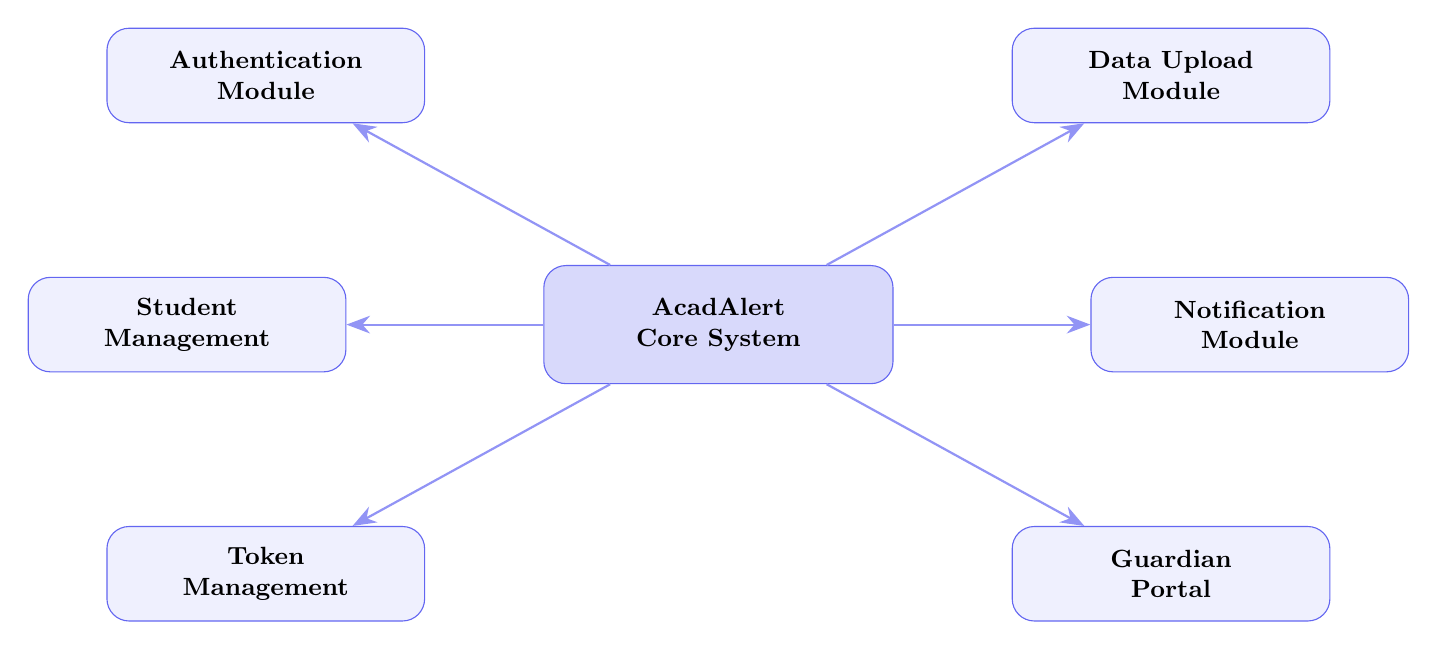
\begin{tikzpicture}[
  module/.style={rectangle, draw=primaryblue, fill=primaryblue!10, rounded corners=8pt, text width=3.8cm, minimum height=1.2cm, align=center, font=\small\bfseries},
  arrow/.style={-{Stealth[length=3mm]}, thick, draw=primaryblue!70}
]
  % Central node
  \node[module, fill=primaryblue!25, text width=4.2cm, minimum height=1.5cm] (core) {AcadAlert\\Core System};

  % Modules
  \node[module, above left=1.8cm and 1.5cm of core] (auth) {Authentication\\Module};
  \node[module, above right=1.8cm and 1.5cm of core] (upload) {Data Upload\\Module};
  \node[module, left=2.5cm of core] (student) {Student\\Management};
  \node[module, right=2.5cm of core] (notify) {Notification\\Module};
  \node[module, below left=1.8cm and 1.5cm of core] (token) {Token\\Management};
  \node[module, below right=1.8cm and 1.5cm of core] (guardian) {Guardian\\Portal};

  % Arrows
  \draw[arrow] (core) -- (auth);
  \draw[arrow] (core) -- (upload);
  \draw[arrow] (core) -- (student);
  \draw[arrow] (core) -- (notify);
  \draw[arrow] (core) -- (token);
  \draw[arrow] (core) -- (guardian);
\end{tikzpicture}
\captionof{figure}{System Module Architecture}
\end{center}

\subsection{Module 1: Authentication Module}
\begin{itemize}
  \item Admin login with email/password verification.
  \item Form validation using React Hook Form with real-time error feedback.
  \item Session management and route protection.
\end{itemize}

\subsection{Module 2: Data Upload Module}
\begin{itemize}
  \item Accepts CSV and Excel files for bulk student data import.
  \item Drag-and-drop interface with file type validation.
  \item Course and branch selection with dynamic dropdown mapping.
  \item Preview of parsed records before submission.
\end{itemize}

\subsection{Module 3: Student Management Module}
\begin{itemize}
  \item Searchable student list with grid/list view toggle.
  \item Filters by branch, semester, and SGPA range.
  \item Detailed student profile with semester-wise mark breakdown.
  \item Interactive SGPA trend chart (LineChart via Recharts).
  \item Detention status highlighting.
\end{itemize}

\subsection{Module 4: Notification Module}
\begin{itemize}
  \item Multi-select students for batch notification dispatch.
  \item Email notification via Nodemailer (Gmail SMTP).
  \item HTML email template with branded ``View Report'' button.
  \item Dynamic URL generation with unique student identifier.
\end{itemize}

\subsection{Module 5: Token Management Module}
\begin{itemize}
  \item Tracks all generated access tokens.
  \item Display of token status (Active, Expired, Revoked).
  \item One-click token revocation and link copying.
  \item Access method tracking (Email, WhatsApp, Direct).
\end{itemize}

\subsection{Module 6: Guardian Portal}
\begin{itemize}
  \item Token-based secure access (no login required).
  \item Student profile with academic summary.
  \item Semester-wise collapsible mark tables with pass/detained indicators.
  \item Interactive SGPA trend line chart.
  \item Attendance ring indicator using SVG.
  \item Report download functionality.
\end{itemize}

%% ===========================
%% CHAPTER 4: SOFTWARE DESIGN
%% ===========================
\chapter{Software Design}

\section{System Architecture -- Block Diagram}

\begin{center}
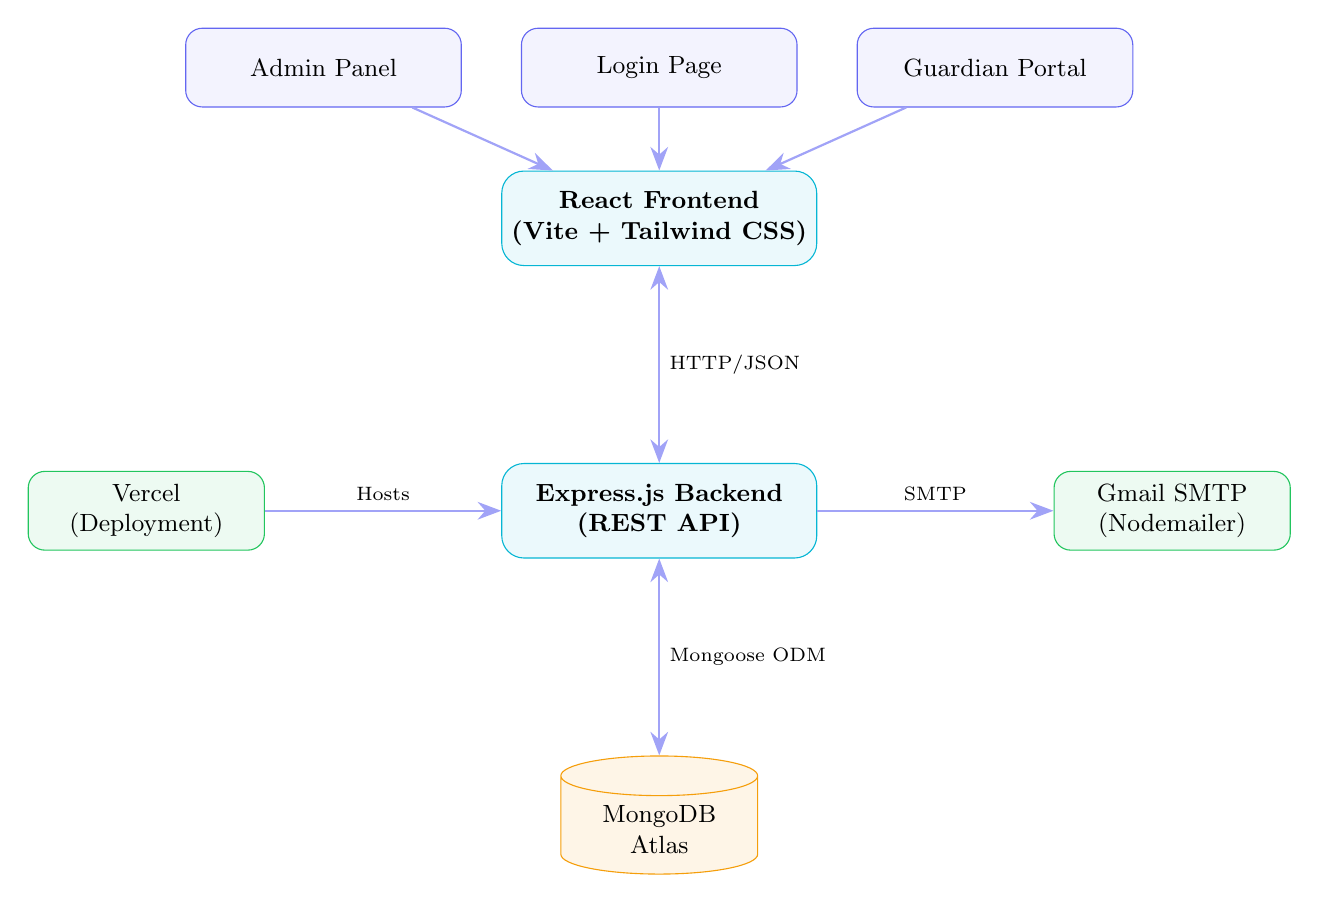
\begin{tikzpicture}[
  block/.style={rectangle, draw=primaryblue, fill=primaryblue!8, rounded corners=6pt, minimum width=3.5cm, minimum height=1cm, align=center, font=\small},
  bigblock/.style={rectangle, draw=accentcyan, fill=accentcyan!8, rounded corners=8pt, minimum width=4cm, minimum height=1.2cm, align=center, font=\small\bfseries},
  dbblock/.style={cylinder, draw=warningamber, fill=warningamber!10, shape border rotate=90, minimum width=2.5cm, minimum height=1.5cm, aspect=0.3, align=center, font=\small},
  extblock/.style={rectangle, draw=successgreen, fill=successgreen!8, rounded corners=6pt, minimum width=3cm, minimum height=1cm, align=center, font=\small},
  arrow/.style={-{Stealth[length=3mm]}, thick, draw=primaryblue!60},
  darrow/.style={{Stealth[length=3mm]}-{Stealth[length=3mm]}, thick, draw=primaryblue!60}
]
  % Frontend
  \node[bigblock] (frontend) {React Frontend\\(Vite + Tailwind CSS)};

  % Backend
  \node[bigblock, below=2.5cm of frontend] (backend) {Express.js Backend\\(REST API)};

  % Database
  \node[dbblock, below=2.5cm of backend] (db) {MongoDB\\Atlas};

  % External Services
  \node[extblock, right=3cm of backend] (email) {Gmail SMTP\\(Nodemailer)};
  \node[extblock, left=3cm of backend] (vercel) {Vercel\\(Deployment)};

  % Sub-components of frontend
  \node[block, above left=0.8cm and 0.5cm of frontend]  (admin)    {Admin Panel};
  \node[block, above right=0.8cm and 0.5cm of frontend] (guardian)  {Guardian Portal};
  \node[block, above=0.8cm of frontend]                 (login)    {Login Page};

  % Arrows
  \draw[arrow] (admin) -- (frontend);
  \draw[arrow] (guardian) -- (frontend);
  \draw[arrow] (login) -- (frontend);
  \draw[darrow] (frontend) -- node[right, font=\scriptsize]  {HTTP/JSON} (backend);
  \draw[darrow] (backend) -- node[right, font=\scriptsize]  {Mongoose ODM} (db);
  \draw[arrow] (backend) -- node[above, font=\scriptsize]  {SMTP} (email);
  \draw[arrow] (vercel) -- node[above, font=\scriptsize]  {Hosts} (backend);
\end{tikzpicture}
\captionof{figure}{System Architecture Block Diagram}
\end{center}

\section{Data Flow Diagram (DFD)}

\subsection{Level 0 -- Context Diagram}

\begin{center}
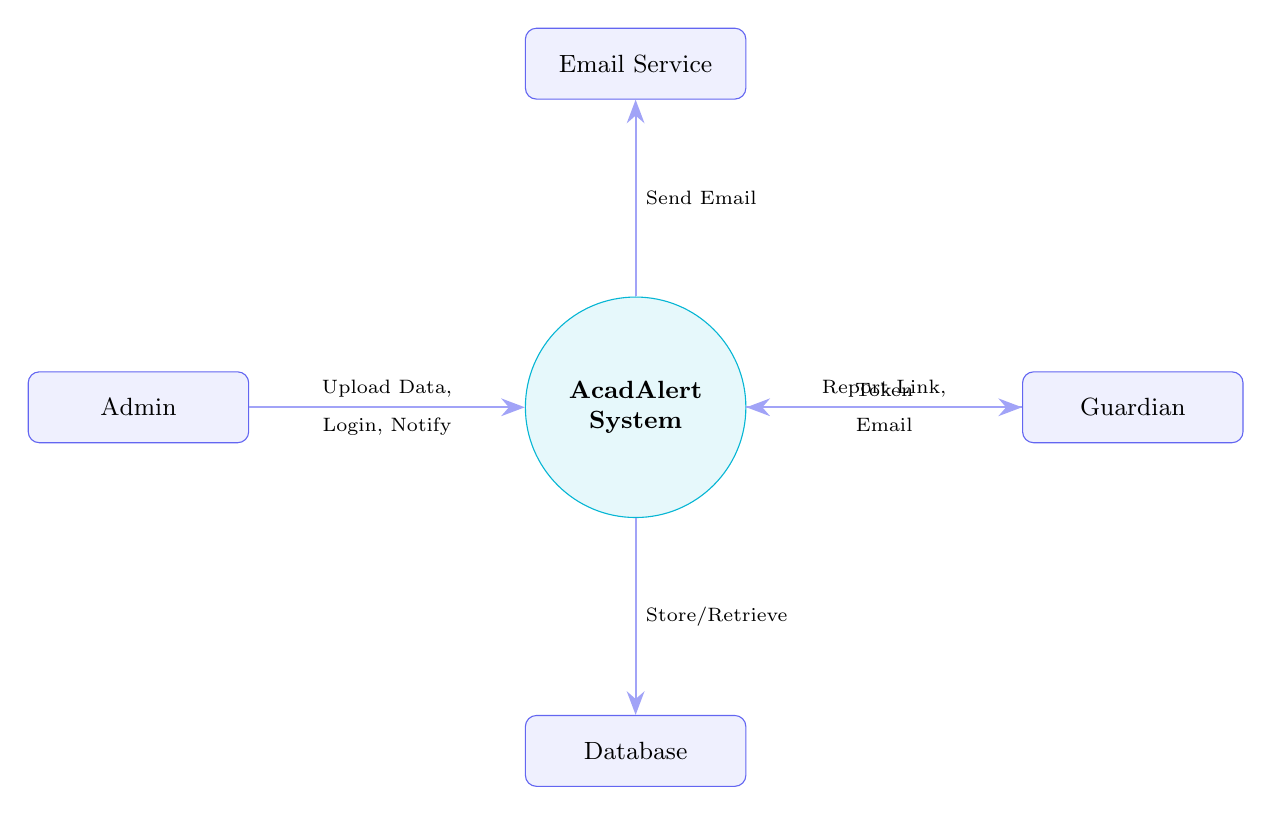
\begin{tikzpicture}[
  entity/.style={rectangle, draw=primaryblue, fill=primaryblue!10, rounded corners=4pt, minimum width=2.8cm, minimum height=0.9cm, align=center, font=\small},
  process/.style={circle, draw=accentcyan, fill=accentcyan!10, minimum size=2.8cm, align=center, font=\small\bfseries},
  arrow/.style={-{Stealth[length=3mm]}, thick, draw=primaryblue!60}
]
  \node[process] (sys) {AcadAlert\\System};
  \node[entity, left=3.5cm of sys] (admin) {Admin};
  \node[entity, right=3.5cm of sys] (guardian) {Guardian};
  \node[entity, below=2.5cm of sys] (db) {Database};
  \node[entity, above=2.5cm of sys] (email) {Email Service};

  \draw[arrow] (admin) -- node[above, font=\scriptsize] {Upload Data,} node[below, font=\scriptsize] {Login, Notify} (sys);
  \draw[arrow] (sys) -- node[above, font=\scriptsize] {Report Link,} node[below, font=\scriptsize] {Email} (guardian);
  \draw[arrow] (guardian) -- node[above, font=\scriptsize, sloped] {Token} (sys);
  \draw[arrow] (sys) -- node[right, font=\scriptsize] {Store/Retrieve} (db);
  \draw[arrow] (sys) -- node[right, font=\scriptsize] {Send Email} (email);
\end{tikzpicture}
\captionof{figure}{Level 0 DFD -- Context Diagram}
\end{center}

\subsection{Level 1 -- DFD}

\begin{center}
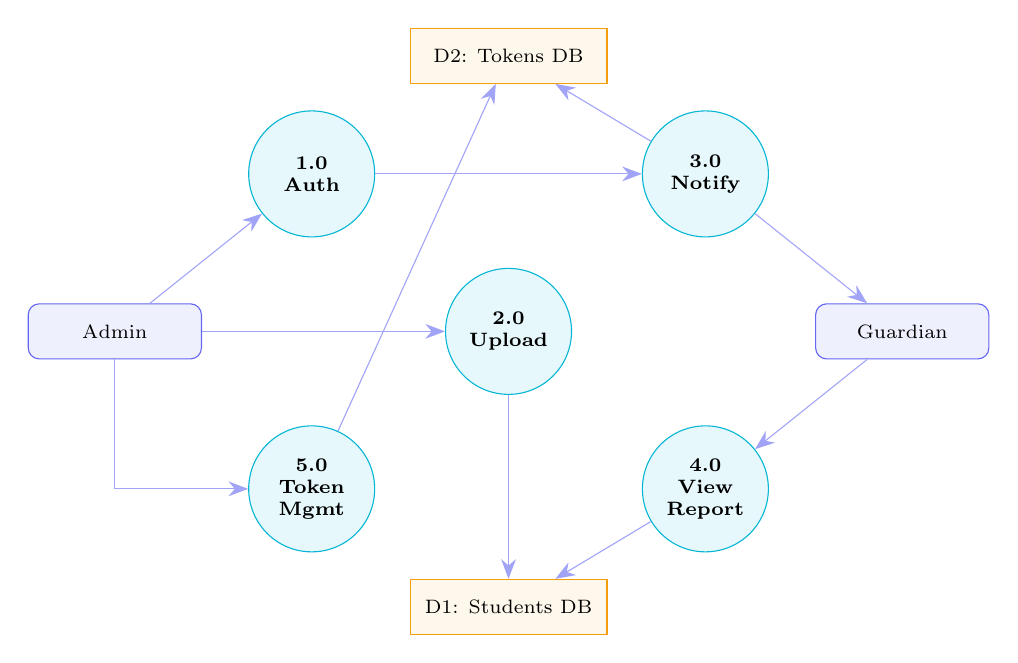
\begin{tikzpicture}[
  entity/.style={rectangle, draw=primaryblue, fill=primaryblue!10, rounded corners=4pt, minimum width=2.2cm, minimum height=0.7cm, align=center, font=\scriptsize},
  process/.style={circle, draw=accentcyan, fill=accentcyan!10, minimum size=1.6cm, align=center, font=\scriptsize\bfseries},
  store/.style={rectangle, draw=warningamber, fill=warningamber!8, minimum width=2.5cm, minimum height=0.7cm, align=center, font=\scriptsize},
  arrow/.style={-{Stealth[length=2.5mm]}, draw=primaryblue!60}
]
  % Entities
  \node[entity] (admin) at (-5,0) {Admin};
  \node[entity] (guardian) at (5,0) {Guardian};

  % Processes
  \node[process] (p1) at (-2.5, 2) {1.0\\Auth};
  \node[process] (p2) at (0, 0) {2.0\\Upload};
  \node[process] (p3) at (2.5, 2) {3.0\\Notify};
  \node[process] (p4) at (2.5, -2) {4.0\\View\\Report};
  \node[process] (p5) at (-2.5, -2) {5.0\\Token\\Mgmt};

  % Data stores
  \node[store] (ds1) at (0, -3.5) {D1: Students DB};
  \node[store] (ds2) at (0, 3.5) {D2: Tokens DB};

  % Arrows
  \draw[arrow] (admin) -- (p1);
  \draw[arrow] (admin) -- (p2);
  \draw[arrow] (p2) -- (ds1);
  \draw[arrow] (p3) -- (guardian);
  \draw[arrow] (guardian) -- (p4);
  \draw[arrow] (p4) -- (ds1);
  \draw[arrow] (p3) -- (ds2);
  \draw[arrow] (p5) -- (ds2);
  \draw[arrow] (admin) |- (p5);
  \draw[arrow] (p1) -- (p3);
\end{tikzpicture}
\captionof{figure}{Level 1 DFD}
\end{center}

\section{Use Case Diagram}

\begin{center}
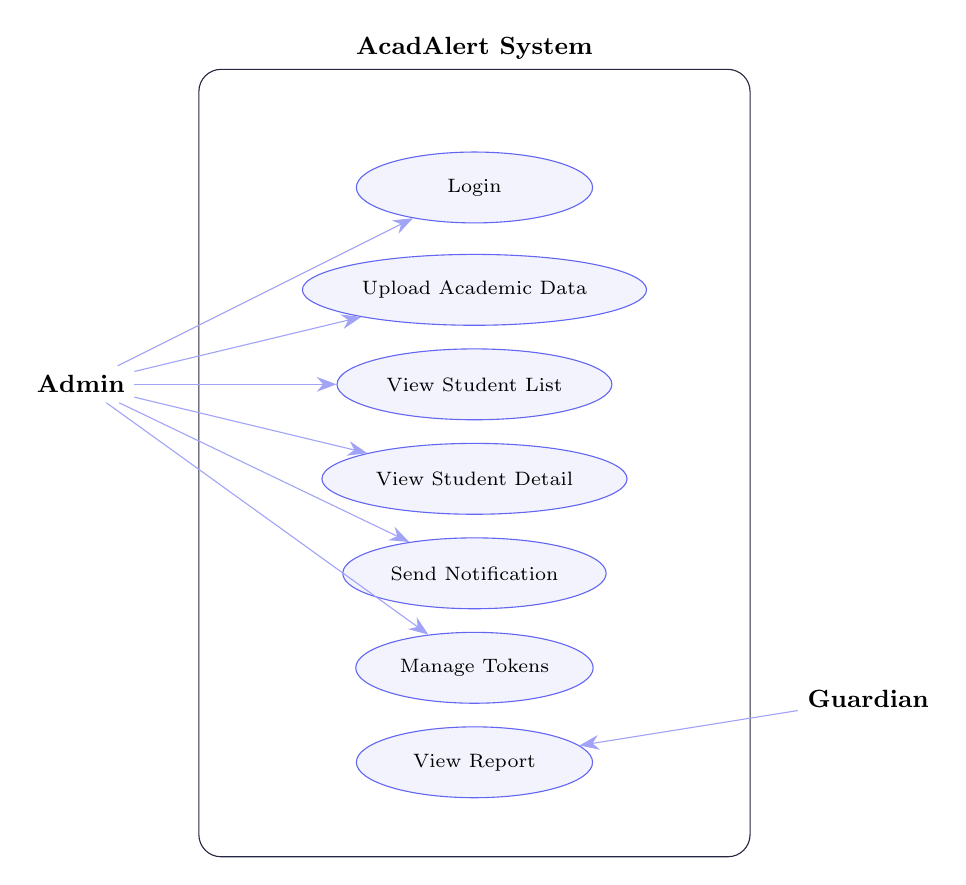
\begin{tikzpicture}[
  actor/.style={font=\small},
  usecase/.style={ellipse, draw=primaryblue, fill=primaryblue!8, minimum width=3cm, minimum height=0.9cm, align=center, font=\scriptsize},
  arrow/.style={-{Stealth[length=2.5mm]}, draw=primaryblue!60},
  sysbox/.style={rectangle, draw=bordercolor, rounded corners=8pt, minimum width=7cm, minimum height=10cm}
]
  % System boundary
  \node[sysbox, label={[font=\small\bfseries]above:AcadAlert System}] (sys) at (0,0) {};

  % Use cases
  \node[usecase] (uc1) at (0, 3.5)  {Login};
  \node[usecase] (uc2) at (0, 2.2)  {Upload Academic Data};
  \node[usecase] (uc3) at (0, 1.0)  {View Student List};
  \node[usecase] (uc4) at (0, -0.2) {View Student Detail};
  \node[usecase] (uc5) at (0, -1.4) {Send Notification};
  \node[usecase] (uc6) at (0, -2.6) {Manage Tokens};
  \node[usecase] (uc7) at (0, -3.8) {View Report};

  % Actors
  \node[actor] (adm) at (-5, 1.0) {\textbf{Admin}};
  \node[actor] (grd) at (5, -3.0)  {\textbf{Guardian}};

  % Admin connections
  \draw[arrow] (adm) -- (uc1);
  \draw[arrow] (adm) -- (uc2);
  \draw[arrow] (adm) -- (uc3);
  \draw[arrow] (adm) -- (uc4);
  \draw[arrow] (adm) -- (uc5);
  \draw[arrow] (adm) -- (uc6);

  % Guardian connections
  \draw[arrow] (grd) -- (uc7);
\end{tikzpicture}
\captionof{figure}{Use Case Diagram}
\end{center}

\section{Sequence Diagram -- Notification Flow}

\begin{center}
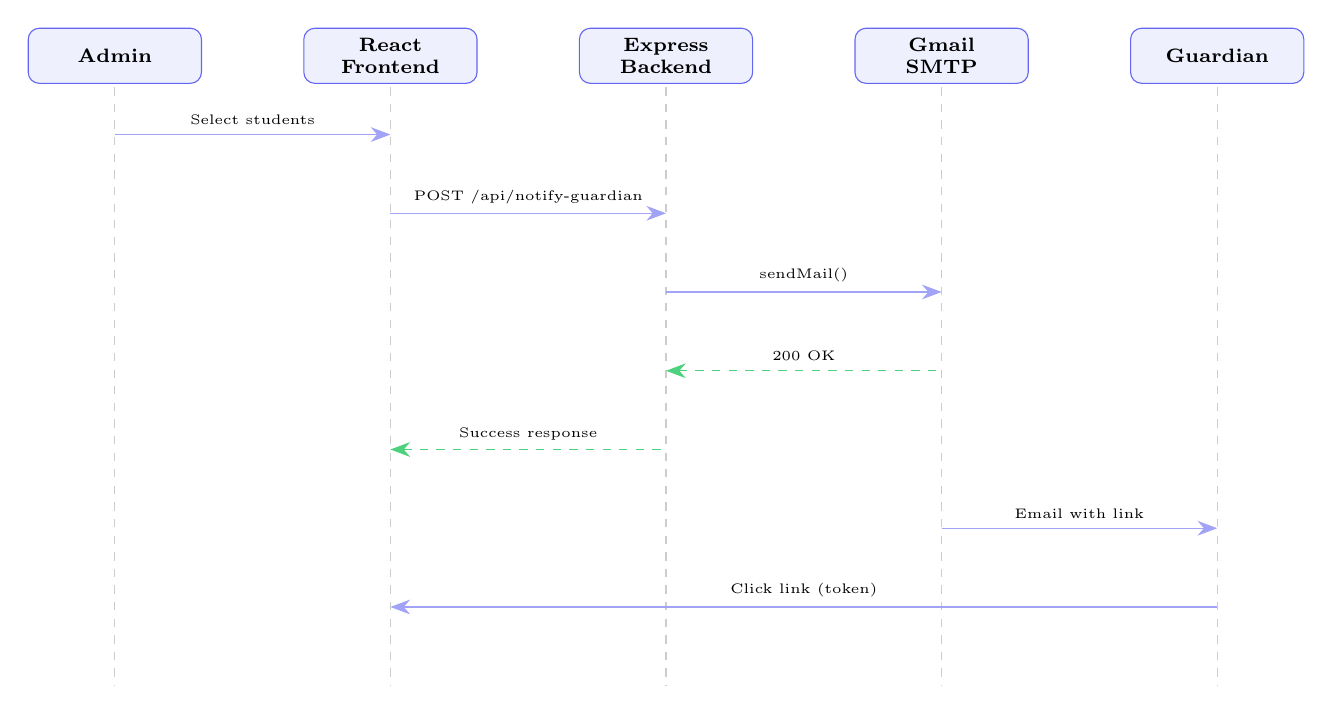
\begin{tikzpicture}[
  box/.style={rectangle, draw=primaryblue, fill=primaryblue!10, rounded corners=4pt, minimum width=2.2cm, minimum height=0.7cm, align=center, font=\scriptsize\bfseries},
  arrow/.style={-{Stealth[length=2.5mm]}, draw=primaryblue!60},
  darrow/.style={{Stealth[length=2.5mm]}-, draw=successgreen!80, dashed}
]
  % Lifelines
  \node[box] (admin) at (0, 0) {Admin};
  \node[box] (frontend) at (3.5, 0) {React\\Frontend};
  \node[box] (backend) at (7, 0) {Express\\Backend};
  \node[box] (smtp) at (10.5, 0) {Gmail\\SMTP};
  \node[box] (guardian) at (14, 0) {Guardian};

  % Lifelines
  \draw[dashed, gray!40] (0, -0.4) -- (0, -8);
  \draw[dashed, gray!40] (3.5, -0.4) -- (3.5, -8);
  \draw[dashed, gray!40] (7, -0.4) -- (7, -8);
  \draw[dashed, gray!40] (10.5, -0.4) -- (10.5, -8);
  \draw[dashed, gray!40] (14, -0.4) -- (14, -8);

  % Messages
  \draw[arrow] (0, -1) -- node[above, font=\tiny] {Select students} (3.5, -1);
  \draw[arrow] (3.5, -2) -- node[above, font=\tiny] {POST /api/notify-guardian} (7, -2);
  \draw[arrow] (7, -3) -- node[above, font=\tiny] {sendMail()} (10.5, -3);
  \draw[darrow] (7, -4) -- node[above, font=\tiny] {200 OK} (10.5, -4);
  \draw[darrow] (3.5, -5) -- node[above, font=\tiny] {Success response} (7, -5);
  \draw[arrow] (10.5, -6) -- node[above, font=\tiny] {Email with link} (14, -6);
  \draw[arrow] (14, -7) -- node[above, font=\tiny] {Click link (token)} (3.5, -7);
\end{tikzpicture}
\captionof{figure}{Sequence Diagram -- Notification Flow}
\end{center}

\section{Activity Diagram -- Admin Workflow}

\begin{center}
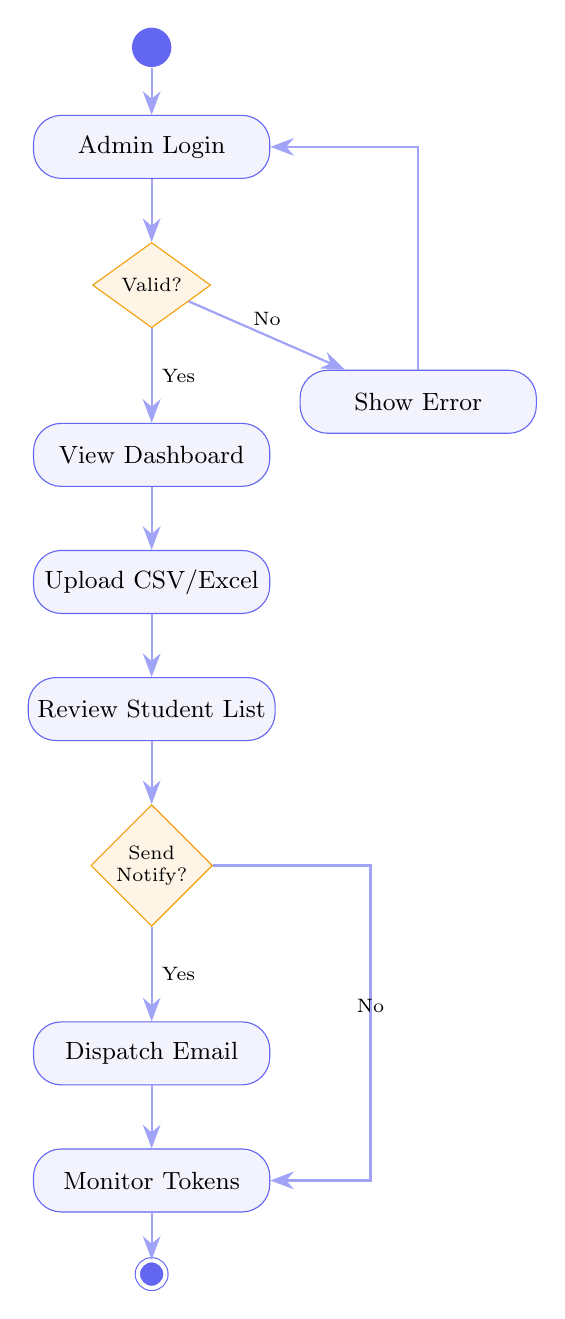
\begin{tikzpicture}[
  start/.style={circle, fill=primaryblue, minimum size=0.5cm},
  stop/.style={circle, draw=primaryblue, fill=primaryblue, minimum size=0.35cm, double, double distance=1.5pt},
  activity/.style={rectangle, draw=primaryblue, fill=primaryblue!8, rounded corners=10pt, minimum width=3cm, minimum height=0.8cm, align=center, font=\small},
  decision/.style={diamond, draw=warningamber, fill=warningamber!10, minimum width=1.5cm, minimum height=1cm, align=center, font=\scriptsize, inner sep=1pt},
  arrow/.style={-{Stealth[length=3mm]}, thick, draw=primaryblue!60}
]
  \node[start] (s) at (0, 0) {};
  \node[activity, below=0.6cm of s] (login) {Admin Login};
  \node[decision, below=0.8cm of login] (d1) {Valid?};
  \node[activity, below right=0.8cm and 1.5cm of d1] (err) {Show Error};
  \node[activity, below=1.2cm of d1] (dash) {View Dashboard};
  \node[activity, below=0.8cm of dash] (upload) {Upload CSV/Excel};
  \node[activity, below=0.8cm of upload] (review) {Review Student List};
  \node[decision, below=0.8cm of review] (d2) {Send\\Notify?};
  \node[activity, below=1.2cm of d2] (notify) {Dispatch Email};
  \node[activity, below=0.8cm of notify] (token) {Monitor Tokens};
  \node[stop, below=0.6cm of token] (e) {};

  \draw[arrow] (s) -- (login);
  \draw[arrow] (login) -- (d1);
  \draw[arrow] (d1) -- node[right, font=\scriptsize] {Yes} (dash);
  \draw[arrow] (d1) -- node[above, font=\scriptsize] {No} (err);
  \draw[arrow] (err) |- (login);
  \draw[arrow] (dash) -- (upload);
  \draw[arrow] (upload) -- (review);
  \draw[arrow] (review) -- (d2);
  \draw[arrow] (d2) -- node[right, font=\scriptsize] {Yes} (notify);
  \draw[arrow] (d2.east) -| ++(2, 0) |- node[above, font=\scriptsize, near start] {No} (token);
  \draw[arrow] (notify) -- (token);
  \draw[arrow] (token) -- (e);
\end{tikzpicture}
\captionof{figure}{Activity Diagram -- Admin Workflow}
\end{center}

\section{Database Design}

\subsection{Entity-Relationship (ER) Diagram}

\begin{center}
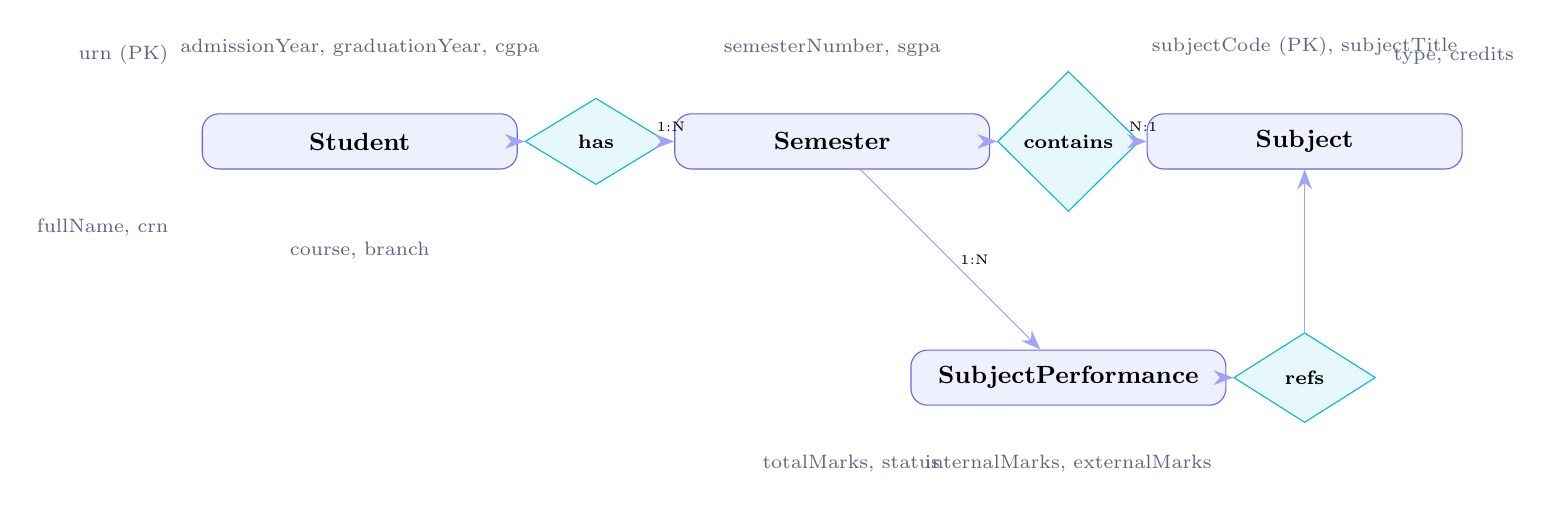
\begin{tikzpicture}[
  entity/.style={rectangle, draw=primaryblue, fill=primaryblue!10, rounded corners=6pt, minimum width=4cm, minimum height=0.7cm, align=center, font=\small\bfseries},
  attr/.style={font=\scriptsize, text=textmuted},
  rel/.style={diamond, draw=accentcyan, fill=accentcyan!10, minimum width=1.8cm, minimum height=1cm, align=center, font=\scriptsize\bfseries},
  arrow/.style={-{Stealth[length=2.5mm]}, draw=primaryblue!60}
]
  % Entities
  \node[entity] (student) at (0, 0) {Student};
  \node[entity] (semester) at (6, 0) {Semester};
  \node[entity] (subject) at (12, 0) {Subject};
  \node[entity] (performance) at (9, -3) {SubjectPerformance};

  % Relationships
  \node[rel] (r1) at (3, 0) {has};
  \node[rel] (r2) at (9, 0) {contains};
  \node[rel] (r3) at (12, -3) {refs};

  % Attributes for Student
  \node[attr, above left=0.5cm and 0.3cm of student] {urn (PK)};
  \node[attr, below left=0.5cm and 0.3cm of student] {fullName, crn};
  \node[attr, below=0.8cm of student] {course, branch};
  \node[attr, above=0.6cm of student] {admissionYear, graduationYear, cgpa};

  % Attributes for Semester
  \node[attr, above=0.6cm of semester] {semesterNumber, sgpa};

  % Attributes for Subject
  \node[attr, above=0.6cm of subject] {subjectCode (PK), subjectTitle};
  \node[attr, above right=0.5cm and -1cm of subject] {type, credits};

  % Attributes for Performance
  \node[attr, below=0.5cm of performance] {internalMarks, externalMarks};
  \node[attr, below left=0.5cm and -0.5cm of performance] {totalMarks, status};

  % Arrows
  \draw[arrow] (student) -- (r1);
  \draw[arrow] (r1) -- node[above, font=\tiny] {1:N} (semester);
  \draw[arrow] (semester) -- (r2);
  \draw[arrow] (r2) -- node[above, font=\tiny] {N:1} (subject);
  \draw[arrow] (performance) -- (r3);
  \draw[arrow] (r3) -- (subject);
  \draw[arrow] (semester) -- node[right, font=\tiny] {1:N} (performance);
\end{tikzpicture}
\captionof{figure}{Entity-Relationship Diagram}
\end{center}

\subsection{Database Schema Details}

\textbf{Student Collection:}
\begin{longtable}{|l|l|p{5.5cm}|}
\hline
\textbf{Field} & \textbf{Type} & \textbf{Description}\\
\hline
fullName & String & Student's full name (required, trimmed)\\
\hline
urn & Number & University Roll Number (unique, required)\\
\hline
crn & Number & Class Roll Number (required)\\
\hline
course & String & Course enrolled (validated against courseBranchMap)\\
\hline
branch & String & Branch of study (validated per course)\\
\hline
admissionYear & Number & Year of admission (min: 2000)\\
\hline
graduationYear & Number & Expected graduation year ($>$ admissionYear)\\
\hline
semesters & Array & Array of Semester sub-documents\\
\hline
cgpa & Number & Auto-calculated after all semesters complete\\
\hline
\end{longtable}

\textbf{Subject Collection:}
\begin{longtable}{|l|l|p{5.5cm}|}
\hline
\textbf{Field} & \textbf{Type} & \textbf{Description}\\
\hline
subjectCode & String & Unique code (uppercase, trimmed)\\
\hline
subjectTitle & String & Full subject name\\
\hline
type & String & ``T'' (Theory) or ``P'' (Practical)\\
\hline
credits & Number & Credit weight of the subject\\
\hline
maxInternalMarks & Number & Maximum internal marks\\
\hline
maxExternalMarks & Number & Maximum external marks\\
\hline
maxTotalMarks & Number & $\geq$ maxInternal + maxExternal\\
\hline
minInternalPassMarks & Number & Minimum to pass internally\\
\hline
minExternalPassMarks & Number & Minimum to pass externally\\
\hline
minTotalPassMarks & Number & $\leq$ maxTotalMarks\\
\hline
\end{longtable}

\section{Component Diagram -- Frontend Architecture}

\begin{center}
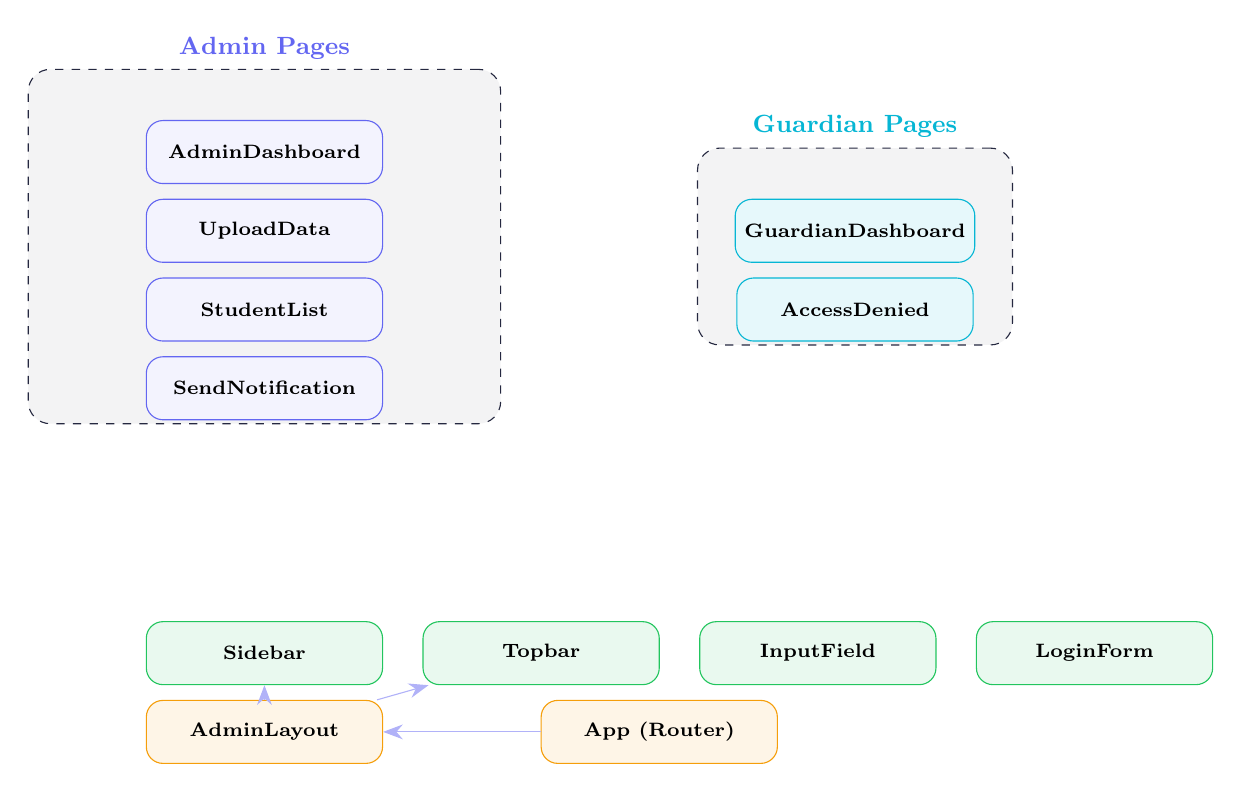
\begin{tikzpicture}[
  comp/.style={rectangle, draw=primaryblue, fill=primaryblue!8, rounded corners=6pt, minimum width=3cm, minimum height=0.8cm, align=center, font=\scriptsize\bfseries},
  pkg/.style={rectangle, draw=bordercolor, dashed, rounded corners=8pt, inner sep=10pt, fill=cardbg!5},
  arrow/.style={-{Stealth[length=2.5mm]}, draw=primaryblue!50}
]
  % Packages
  \node[pkg, minimum width=6cm, minimum height=4.5cm, label={[font=\small\bfseries, text=primaryblue]above:Admin Pages}] (adminpkg) at (-3.5, 0) {};
  \node[pkg, minimum width=4cm, minimum height=2.5cm, label={[font=\small\bfseries, text=accentcyan]above:Guardian Pages}] (guardpkg) at (4, 0) {};

  % Admin components
  \node[comp] (adash) at (-3.5, 1.2) {AdminDashboard};
  \node[comp] (aupload) at (-3.5, 0.2) {UploadData};
  \node[comp] (alist) at (-3.5, -0.8) {StudentList};
  \node[comp] (anotify) at (-3.5, -1.8) {SendNotification};

  % Guardian components
  \node[comp, fill=accentcyan!10, draw=accentcyan] (gdash) at (4, 0.2) {GuardianDashboard};
  \node[comp, fill=accentcyan!10, draw=accentcyan] (gaccess) at (4, -0.8) {AccessDenied};

  % Shared
  \node[comp, below=2.5cm of adminpkg, fill=successgreen!10, draw=successgreen] (sidebar) {Sidebar};
  \node[comp, right=0.5cm of sidebar, fill=successgreen!10, draw=successgreen] (topbar) {Topbar};
  \node[comp, right=0.5cm of topbar, fill=successgreen!10, draw=successgreen] (input) {InputField};
  \node[comp, right=0.5cm of input, fill=successgreen!10, draw=successgreen] (loginform) {LoginForm};

  % Layout
  \node[comp, below=3.5cm of adminpkg, fill=warningamber!10, draw=warningamber] (layout) {AdminLayout};
  \node[comp, right=2cm of layout, fill=warningamber!10, draw=warningamber] (router) {App (Router)};

  \draw[arrow] (layout) -- (sidebar);
  \draw[arrow] (layout) -- (topbar);
  \draw[arrow] (router) -- (layout);
\end{tikzpicture}
\captionof{figure}{Frontend Component Architecture}
\end{center}

\section{Deployment Diagram}

\begin{center}
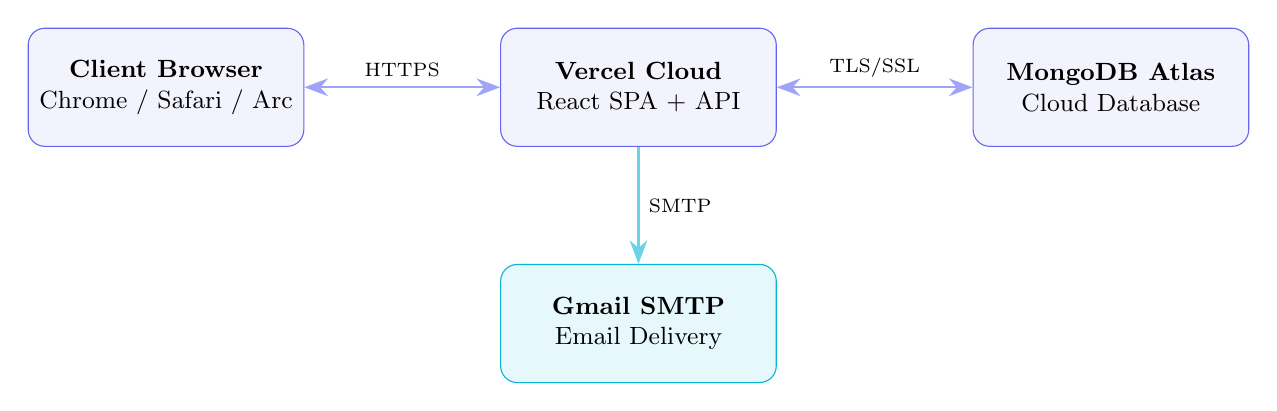
\begin{tikzpicture}[
  node3d/.style={rectangle, draw=primaryblue, fill=primaryblue!8, rounded corners=6pt, minimum width=3.5cm, minimum height=1.5cm, align=center, font=\small},
  arrow/.style={{Stealth[length=3mm]}-{Stealth[length=3mm]}, thick, draw=primaryblue!60}
]
  \node[node3d] (client) at (0, 0) {\textbf{Client Browser}\\Chrome / Safari / Arc};
  \node[node3d] (vercel) at (6, 0) {\textbf{Vercel Cloud}\\React SPA + API};
  \node[node3d] (atlas) at (12, 0) {\textbf{MongoDB Atlas}\\Cloud Database};
  \node[node3d, fill=accentcyan!10, draw=accentcyan] (gmail) at (6, -3) {\textbf{Gmail SMTP}\\Email Delivery};

  \draw[arrow] (client) -- node[above, font=\scriptsize] {HTTPS} (vercel);
  \draw[arrow] (vercel) -- node[above, font=\scriptsize] {TLS/SSL} (atlas);
  \draw[-{Stealth[length=3mm]}, thick, draw=accentcyan!60] (vercel) -- node[right, font=\scriptsize] {SMTP} (gmail);
\end{tikzpicture}
\captionof{figure}{Deployment Diagram}
\end{center}

%% ===========================
%% CHAPTER 5: TESTING MODULE
%% ===========================
\chapter{Testing Module}

\section{Testing Approach}

The system is tested using a combination of manual functional testing, integration testing, and cross-browser validation. The testing strategy covers:

\begin{enumerate}
  \item \textbf{Unit-Level Validation}: Mongoose schema validators (marks ranges, course-branch mapping, CGPA calculation).
  \item \textbf{API Testing}: REST endpoint testing using Postman/Thunder Client.
  \item \textbf{UI/UX Testing}: Manual browser testing on Chrome, Safari, and Arc.
  \item \textbf{Cross-Device Testing}: Responsive layout verification on desktop and mobile viewports.
  \item \textbf{Email Delivery Testing}: Verifying Gmail SMTP delivery and HTML template rendering.
\end{enumerate}

\section{Test Cases}

\begin{longtable}{|p{0.5cm}|p{3cm}|p{4.5cm}|p{2cm}|p{2cm}|}
\hline
\textbf{ID} & \textbf{Test Case} & \textbf{Steps} & \textbf{Expected} & \textbf{Result}\\
\hline
\endfirsthead
TC1 & Admin Login -- Valid & Enter admin@acadm.edu / admin123, click Submit & Redirect to Dashboard & \textcolor{successgreen}{Pass}\\
\hline
TC2 & Admin Login -- Invalid & Enter wrong credentials, click Submit & Error message displayed & \textcolor{successgreen}{Pass}\\
\hline
TC3 & Login Form Validation & Submit empty form & Required field errors shown & \textcolor{successgreen}{Pass}\\
\hline
TC4 & Email Regex Validation & Enter non-Gmail address & Pattern error shown & \textcolor{successgreen}{Pass}\\
\hline
TC5 & CSV Upload & Upload valid CSV file & Records parsed and previewed & \textcolor{successgreen}{Pass}\\
\hline
TC6 & Invalid File Upload & Upload .txt file & Rejection with error & \textcolor{successgreen}{Pass}\\
\hline
TC7 & Student Search & Type name in search bar & Filtered list displayed & \textcolor{successgreen}{Pass}\\
\hline
TC8 & View Student Detail & Click student card & Detail page with charts loads & \textcolor{successgreen}{Pass}\\
\hline
TC9 & Send Notification & Select students, click Send & API call, success message & \textcolor{successgreen}{Pass}\\
\hline
TC10 & Guardian Token Access & Open link with valid token & Student report displayed & \textcolor{successgreen}{Pass}\\
\hline
TC11 & Invalid Token Access & Open link with invalid token & Access Denied page shown & \textcolor{successgreen}{Pass}\\
\hline
TC12 & Token Revocation & Click Revoke on active token & Token status changes to Revoked & \textcolor{successgreen}{Pass}\\
\hline
TC13 & SGPA Chart Rendering & View student detail page & Line chart with all semesters renders & \textcolor{successgreen}{Pass}\\
\hline
TC14 & Responsive Layout & Resize browser to mobile width & Layout adapts, sidebar collapses & \textcolor{successgreen}{Pass}\\
\hline
TC15 & Email HTML Rendering & Receive notification email & Branded template with button renders & \textcolor{successgreen}{Pass}\\
\hline
\end{longtable}

%% ===========================
%% CHAPTER 6: PERFORMANCE
%% ===========================
\chapter{Performance of the Project Developed (So Far)}

\section{Development Progress}

\begin{center}
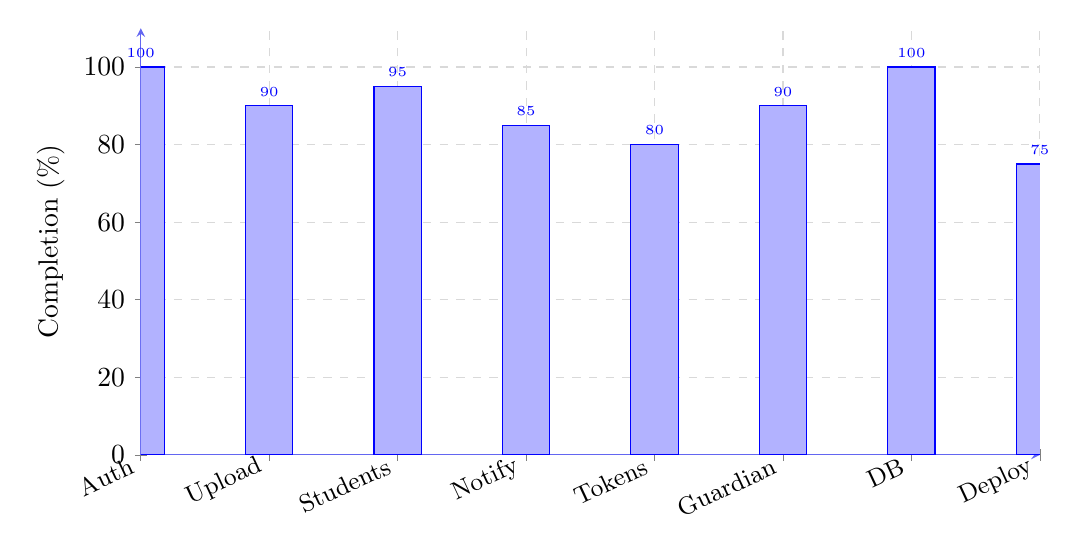
\begin{tikzpicture}
\begin{axis}[
  ybar,
  width=13cm, height=7cm,
  bar width=0.6cm,
  ylabel={Completion (\%)},
  symbolic x coords={Auth, Upload, Students, Notify, Tokens, Guardian, DB, Deploy},
  xtick=data,
  x tick label style={rotate=25, anchor=east, font=\small},
  ymin=0, ymax=110,
  nodes near coords,
  nodes near coords style={font=\tiny},
  axis lines=left,
  grid=major,
  grid style={dashed, gray!30},
  fill=primaryblue!60,
  draw=primaryblue,
]
\addplot coordinates {
  (Auth, 100) (Upload, 90) (Students, 95) (Notify, 85) (Tokens, 80) (Guardian, 90) (DB, 100) (Deploy, 75)
};
\end{axis}
\end{tikzpicture}
\captionof{figure}{Module-wise Development Progress}
\end{center}

\section{Key Metrics}

\begin{longtable}{|p{5.5cm}|p{7.5cm}|}
\hline
\textbf{Metric} & \textbf{Value}\\
\hline
Total Students in Test DB & 248\\
\hline
Notifications Dispatched & 192\\
\hline
Detained Students Tracked & 18\\
\hline
Active Access Tokens & 34\\
\hline
Courses Supported & 9 (B.Tech, M.Tech, MBA, MCA, BCA, B.Arch, B.Voc., B.Com, BBA)\\
\hline
Average CGPA (Institution) & 7.84\\
\hline
Frontend Components & 12+\\
\hline
Backend API Endpoints & RESTful (POST /api/notify-guardian)\\
\hline
Email Delivery Success Rate & $>$95\%\\
\hline
Development Period & Sept 2025 -- March 2026\\
\hline
\end{longtable}

\section{Challenges Faced}

\begin{enumerate}
  \item \textbf{Safari Timer Bug}: JavaScript timers pause when Safari opens a new tab (e.g., WhatsApp link). Resolved by using \texttt{visibilitychange} event listener instead of \texttt{setTimeout}.
  \item \textbf{CORS in Production}: Vercel serverless functions required explicit CORS origin configuration with credentials enabled.
  \item \textbf{MongoDB Atlas Free Tier}: Limited to 10 concurrent connections; resolved by implementing connection pooling with \texttt{maxPoolSize: 10}.
  \item \textbf{Email Deliverability}: Initial emails landing in spam; resolved by using Gmail App Passwords and proper ``From'' headers.
\end{enumerate}

%% ===========================
%% CHAPTER 7: OUTPUT SCREENS
%% ===========================
\chapter{Output Screens}

\textit{The following screens represent the current state of the AcadAlert system. Screenshots are to be added from the running application.}

\vspace{0.5cm}

\begin{enumerate}
  \item \textbf{Login Page} -- Dark-themed admin login with email/password fields, React Hook Form validation, gradient logo, and grid background.

  \item \textbf{Admin Dashboard} -- Stat cards (Total Students, Notifications Sent, Detained, Active Tokens, Average CGPA), Area chart for notification activity, Bar chart for branch distribution, Recent uploads table.

  \item \textbf{Upload Data} -- Course/branch/semester selection dropdowns, drag-and-drop CSV/Excel upload zone, parsed data preview table.

  \item \textbf{Student List} -- Searchable grid/list view with SGPA colour coding, branch filter, click-to-navigate to detail.

  \item \textbf{Student Detail} -- Student profile header, SGPA trend line chart, semester-wise collapsible tables showing internal/external marks and detention flags.

  \item \textbf{Send Notification} -- Multi-select student table, dispatch button with success/failure feedback.

  \item \textbf{Token Management} -- Token table with status badges (Active/Expired/Revoked), access method tags, revoke and copy-link actions.

  \item \textbf{Guardian Dashboard} -- Token-authenticated view with student summary, SGPA chart, semester breakdown tables, attendance ring, and download report button.

  \item \textbf{Access Denied Page} -- Shown when token is invalid/expired/revoked.

  \item \textbf{Email Template} -- Branded HTML email with ``View Report'' CTA button.
\end{enumerate}

\textit{[Insert screenshots here]}

%% ===========================
%% CHAPTER 8: REFERENCES
%% ===========================
\chapter{References}

\begin{enumerate}
  \item React Documentation -- \url{https://react.dev/}
  \item Express.js v5 Documentation -- \url{https://expressjs.com/}
  \item MongoDB Documentation -- \url{https://www.mongodb.com/docs/}
  \item Mongoose ODM Documentation -- \url{https://mongoosejs.com/docs/}
  \item Nodemailer Documentation -- \url{https://nodemailer.com/}
  \item Tailwind CSS v4 Documentation -- \url{https://tailwindcss.com/docs}
  \item Recharts Documentation -- \url{https://recharts.org/en-US/}
  \item React Hook Form Documentation -- \url{https://react-hook-form.com/}
  \item Vite Build Tool -- \url{https://vitejs.dev/}
  \item Lucide Icons -- \url{https://lucide.dev/}
  \item Vercel Deployment Platform -- \url{https://vercel.com/docs}
  \item React Router v7 -- \url{https://reactrouter.com/}
  \item Minor Project Synopsis -- Group G14, Department of CSE, GNDEC Ludhiana.
\end{enumerate}

\end{document}
